\chapter{Imlementación JPEG}\label{ch:implementacion}

Se implementó un codificador JPEG, lanzado al dominio público en github bajo el
nombre de TinyJPEG \cite{tiny_jpeg}. La ubicación permanente de esta biblioteca
está en \begin{alltt}https://github.com/serge-rgb/TinyJPEG \end{alltt}

Encima de TinyJPEG, se desarrolló un proyecto que extiende TinyJPEG para
implementar el algoritmo evolutivo \cite{gp_encoder}, localizado en
\begin{alltt}https://github.com/serge-rgb/gp_encoder\end{alltt}

En este capítulo se describen los detalles de ambos proyectos.

\section {Términos}
Se van a usar los términos \emph{debugging} y \emph{profiling} por su ubiquidad
en la literatura. \emph{debugging} se traduce como depurar y se define como el
proceso de encontrar y arreglar defectos de código. \emph{profiling} es el
proceso de encontrar los puntos en los que un programa puede ser modificado
para mejorar el desempeño.

\emph{General Purpose GPU}, o \emph{GPGPU} es el
término usado para la práctica de usar programar GPUs directamente, a
diferencia de el uso original, en el cual el GPU era un acelerador cuya
interfaz era una biblioteca de gráficas como OpenGL o DirectX.

% ============================================================
\section{Tecnologías}
% ============================================================

La elección de lenguaje para TinyJPEG fue C. C99 para ser específico
\cite{c99}. TinyJPEG fue lanzado con el objetivo de ser una biblioteca
reutilizable por otras personas, y ha encontrado cierto grado de éxito. Un
planetario en París usa TinyJPEG para capturar vídeo de sus simulaciones.

C es un lenguaje ideal para escribir cosas como codificadores. El lenguaje
permite mantener el nivel bajo de abstracción que se necesita y las
herramientas de \emph{debugging} son mejores para C y C++ que para casi
cualquier otro lenguaje.

Se escogió OpenCL para la implementación de GPGPU. OpenCL es un estándar abierto
para GPGPU y está soportado por Intel, Nvidia y AMD. La máquina en la que se
implementó este trabajo tiene una tarjeta Nvidia. Nvidia tiene su propio
lenguaje para GPGPU, llamado CUDA, que tiene mejor soporte para debugging y
profiling que OpenCL para sus tarjetas de video. Sin embargo, las herramientas
siguen siendo primitivas comparadas con lo que se tiene en el CPU. En cualquier
caso, uno termina haciendo hipótesis, experimentos y medidas para optimizar la
solución, aún teniendo herramientas sofisticadas. Se escogió OpenCL porque los
méritos relativos de facilidad de desarrollo no le ganan al soporte
multi-plataforma y al valor de apoyar estándares abiertos.

% ============================================================
\section{Arquitectura}
% ============================================================

TinyJPEG es minimalista. Consiste de un archivo de alrededor 1000 líneas. Está
escrito en el estilo popularizado por Sean Barrett de escribir un solo archivo
\verb+.h+ con la siguiente estructura:

\label{alg:stb}
\begin{code}[language=C][h]
    // Principio del archivo
    #pragma once

    // Definición de la interfaz.
    tje_encode_to_file(...);

    #ifdef TJE_IMPLEMENTATION

    // La implementación completa va aquí.
\end{code}

De esta manera, uno puede incluir \verb+#include <tiny_jpeg.h>+ como cualquier
\emph{header} de C, pero en uno de los archivos del proyecto, se hace esto:

\label{alg:stb_impl}
\begin{code}[language=C][h]
    #define TJE_IMPLEMENTATION
    #include <tiny_jpeg.h>
\end{code}

para definir la implementación completa. El propósito de esta técnica es
facilitar la distribución de bibliotecas en un lenguaje que no cuenta con un
sistema de distribución digital de módulos,
o siquiera un sistema de módulos.

Se exponen dos funciones como interfaz pública:

\begin{code}[language=C][h]
tje_encode_to_file(...)
tje_encode_to_file_at_quality(...)
\end{code}

La primera comprime con la tabla unitaria y la segunda ofrece tres posibles
niveles de calidad: "alto", "mediano", y "bajo". Todos correspondientes
únicamente al uso de tres tablas de cuantificación.

Ambas funciones son \emph{wrappers} sobre la función principal
interna, que funciona de la siguiente manera:

Se prepara una estructura estática para hacer compresión de Huffman y se
pre-procesa la tabla según el algoritmo dct descrito en \ref{sec:DCT}. A esto
le llamamos el \emph{paso inicial}.  Cuando terminamos el \emph{paso inicial},
determinamos el número de bloques que van a ser procesados. JPEG debe funcionar
con imágenes cuyos tamaños verticales y horizontales no son múltiplos de 8.
Para esto la especificación sólo nos pide como codificador redondear al
siguiente múltiplo de 8. Al decodificador le pide ignorar los datos extra. Para
evitar artefactos, como convención se repite en el bloque el color del último
píxel de la imagen para cada columna extra y para cada renglón extra. Si $w$ es
el ancho de la imagen y $h$ es el alto, entonces el número de bloques es $n =
(w + (8 - w \mod 8)) * (h + (8 - h \mod 8))$

Cada bloque se separa en tres bloques \verb+Y+, \verb+U+ \verb+V+ que a los que
se les aplica la función \verb+encode_MCU()+.

La función \verb+encode_MCU()+ es llamada así por el acrónimo \emph{MCU},
\emph{Minimum Coded Unit}. JPEG puede especificar un factor para describir los
bloques \verb+U+ y \verb+V+ con menos resolución, por nuestra relativa falta de
sensibilidad a la crominancia contra la luminancia, pero TinyJPEG no utiliza
esto. Otra posibilidad es usar diferentes tablas de codificación para
lumninancia y crominancia. TinyJPEG sí utiliza esto, escogiendo tablas con
mayor compresión para los bloques de crominancia.

El flujo de la lógica es parecido a como se describe en Español.
Un \verb+for loop+ para extraer los bloques, y cada bloque se pasa como
parámetro a la función \verb+encode_MCU+.

\subsection{DummyJPEG} \label{sub:dummy}

A primera vista, el algoritmo JPEG se ve ``embarazosamente paralelo". Una
motivación para este trabajo fue la observación de que el algoritmo trabaja
dividiendo la imágenes en cuadros de $8\times8$, y el hecho de que los GPUs
actuales trabajan con instrucciones vectoriales de 64 elementos.

Desafortunadamente, el algoritmo JPEG no es paralelo. Aplicar codificación
delta al coeficiente DC introduce una dependencia de datos entre cada bloque de
\verb+Y+, \verb+U+ y \verb+V+ respectivamente. Para cada componente, cualquier
bloque después del primero depende del anterior para poder computar la
diferencia entre su coeficiente DC  y el de su antecesor.

Sin embargo, aunque JPEG es inherentemente secuencial para cada componente,
está muy cerca de ser paralelo. Si el \emph{Joint Photographic Experts Group}
no hubiera decidido tratar de manera diferente a los coeficientes DC y AC, el
algoritmo sería completamente paralelo.

Queremos darle la vuelta al problema, y la manera en que lo hacemos es creando
un "Dummy JPEG": Un algoritmo que es \emph{casi} JPEG, pero que no es correcto.

La implementación de DummyJPEG empieza como un clon directo de TinyJPEG. Lo
primero que hacemos es cambiar las función que escribe a disco por una función
que va contando el número de bits. De esta manera, al aplicar el algoritmo no
tenemos una imagen, pero tenemos un reporte del tamaño de la imagen que
hubiéramos generado.

También cambiamos el algoritmo para aplicar la Transformada Inversa de Coseno
justo después de aplicar la DCT al bloque, para poder compararlos y calcular el
error.

Entonces, si nuestro algoritmo original para cada bloque en TinyJPEG es:

\begin{code}
    x = aplicar_dct(bloque);
    codificar(x)
\end{code}

Nuestro algoritmo para cada bloque en DummyJPEG se convierte en esto:

\begin{code}
    x = aplicar_dct(bloque)
    reportar_tamaño(x)
    y = aplicar_idct(x)
    reportar_error(bloque, y)
\end{code}

En donde \verb+reportar_error+ es una suma de la diferencia absoluta entre cada
pixel del bloque original y del bloque reconstruido.

La manera en que volvemos paralelo a DummyJPEG es simplemente no codificar al
coeficiente DC. Esto introduce un error en el tamaño reportado pero no afecta
al error reportado. El error que introducimos viene de que contamos los bits de
la representación de los 63 coeficientes AC, pero no contamos los bits del
coeficiente DC. En las imágenes de prueba que se usaron para este trabajo, el
tamaño reportado es menor que el tamaño real entre un 10\% y 20\%. El error es
proporcionalmente más alto para imágenes con más energía en el primer
coeficiente.

La pregunta que nos hacemos es: ¿El error en el reporte de tamaño es
significativo?

Las presión que se pone en la evolución es hacia imágenes que son
indistinguibles de la original. Como el valor de cuantificación del primer
coeficiente afecta de manera importante a la calidad de imagen comprimida, las
tablas de la población rápidamente convergen a tener el primer valor de
cuantificación igual a 1. Esto quiere decir que para casi cualquier conjunto de
tablas que vayamos a comparar, estamos introduciendo el mismo error en el
reporte de los tamaños de las imágenes resultantes. Por lo tanto, podemos
despreocuparnos por completo de no tomar en cuenta el primer coeficiente.

Otra cosa que se hace es \emph{solo calcular bloques de luminancia}. Los
bloques de crominancia usualmente usan una tabla secundaria, y el propósito es
evolucionar una sola tabla. Podemos deshacernos de $66\%$ del trabajo si
descartamos los dos componentes de crominancia. Más tarde, cuando se finalice
la evolución, podemos usar la misma tabla para los tres componentes, o bajar la
calidad de la tabla para los componentes de crominancia multiplicando cada
elemento por alguna constante.

% Describir el deseo de hacer una implementación paralela en el CPU
Ya que tenemos un algoritmo que es \emph{casi JPEG}, pero paralelo, seguimos
con la tarea de cambiar la arquitectura del programa para paralelizarlo en el
CPU. La razón por la que implementamos el paralelismo en el CPU antes de
hacerlo en el GPU es principalmente la velocidad de desarrollo. La manera en
que implementamos la versión paralela en CPU se hace con \emph{plan con maña}.
Moldeamos el código para que el flujo de ejecución en el CPU sea muy
similar a la manera en que trabaja el GPU, intentando llegar al punto de que la
implementación en el GPU se reduzca a un \emph{copy paste}, y que el esfuerzo
que se aplique a la implementación del GPU sea solamente un trabajo de
optimización de bajo nivel.

\section{Introducción a GPGPU}

Las arquitecturas de GPU, en el momento que se escribe esto, trabajan con
instrucciones SIMD (\emph{Single Instruction, Multiple Data}), también llamadas
\emph{instrucciones vectoriales}.

Supercomputadoras vectoriales como la \emph{Cray} se introdujeron en los 70s y
gradualmente perdieron popularidad mientras computadoras con microprocesadores
x86 bajaron de precio.

En 1998 AMD introdujo instrucciones vectoriales con su tecnología \emph{3D
Now}, seguido por Intel en 1999 cuando introdujo SSE (Streaming SIMD
extensions). Ambas tecnologías son extensiones al conjunto de instrucciones x86.

Por esa misma época empezaron a salir aceleradores gráficos: tarjetas que se
dedicaban a rasterizar triángulos rápidamente para aplicaciones multimedia,
principalmente videojuegos.

Aunque al principio los GPUs estaban diseñados alrededor de APIs como OpenGL y
DirectX, con funcionalidad fija, poco a poco fueron adquiriendo la habilidad de
ser programables. Primero con \emph{shaders}, que permitieron meter código en
un par de partes clave del proceso de rasterización, y más tarde con OpenCL y
CUDA, que permiten escribir programas para el GPU en un dialecto de C.

El modelo de ejecución de OpenCL se mapea directamente a las arquitecturas GPU
actuales y funciona de la siguiente manera.

Un programa OpenCL opera con \emph{work items}. Un work item puede pensarse
como un thread, pero lo que es realmente es una \emph{``fibra"} en un
\emph{``cable"} que ejecuta instrucciones vectoriales. En la arquitecturas
modernas de Nvidia, la longitud de los vectores es de 32 elementos.

A estos \emph{``cable"} se les denomina \emph{wavefronts}.

La tarjeta de video tiene un calendarizador implementado en hardware que
trabaja con granularidad de \emph{wavefronts} individuales.  Los \emph{work
items} corren \emph{kernels}, que son esencialmente funciones escritas en el
dialecto de C de OpenCL para ser ejecutadas en el GPU.

Un \emph{work item} es parte de un \emph{work group}. El tamaño del \emph{work
group} es decisión del programador, puede ser de 1, 2 o 3 dimensiones y su
tamaño puede variar, aunque es buena práctica escoger un múltiplo del tamaño
vectorial (32 en Kepler y Maxwell). Hay que encontrar el tamaño apropiado de
\emph{work group} para minimizar contención de memoria y maximizar el
rendimiento (traducción de \emph{throughput}).

El \emph{work group} es una abstracción que se provee para proveer al
\emph{kernel} con índices relativos a la dimensión y tamaño del espacio de
\emph{work groups}. Esto es útil para que el programador diseñe el algoritmo
para utilizar la jerarquía de memoria eficientemente y evitar ejecución
condicional. Es útil usar referencias oficiales \cite{maxwell-tuning} o buscar
los recursos gratis de GPU Tech Conf, una conferencia anual sobre GPUs en la
que siempre hay pláticas que explican tips y trucos para sacar el mayor
desempeño posible de las arquitecturas actuales. \cite{gtc}


En la microarquitectura del GPU, los \emph{wavefronts} son ejecutados en
procesadores vectoriales llamados \emph{Compute Units}. Cada Compute Unit tiene
un número limitado de registros y un espacio de memoria local (a veces llamada
stack, por su equivalente operacional en CPUs). Cada work group tiene
\emph{memoria compartida}, con acceso de lectura y escritura para cualquier
miembro del grupo. Todos los wavefronts tienen acceso de lectura y escritura a
la memoria global. El CPU también tiene acceso de lectura y escritura al
espacio de memorial global, y es por aqui donde se especifican datos de entrada
para el kernel y de donde se leen los resultados.  Los demás espacios de
memoria sólo son accesibles desde adentro de un kernel.

La arquitectura de los GPUs está diseñada para lidiar con problemas de
contención de memoria. Cuando algún work item dentro de un wavefront está
esperando a que se efectúe una operación de memoria, el calendarizador hace que
el \emph{core} ejecute otro wavefront que esté listo para ser ejecutado.

Hay una correspondencia entre el modelo de memoria de OpenCL y la jerarquía de
memoria de las arquitecturas GPU. Existe una memoria compartida con garantía de
coherencia, y un número de \emph{cores} capaces de ejecutar \emph{work items}
que existen en grupos de tamaño fijo con memoria local. Estos \emph{cores} son
llamados \emph{streaming multiprocessors}, abreviados SMX. El número de SMX
varía por GPU. No esta fijado por la arquitectura. Chips basados en Kepler
pueden tener entre 4 y 14 SMX, cada uno con 192 \emph{cuda cores}. Cada
\emph{cuda core} tiene sus propios registros y puede ejecutar un work item. Todos
los cuda cores en un SMX comparten un cache L1. Todos los SMX comparten un
cache L2. \cite{kepler-notes}.

El kernel para nuestra función de selección va a hacer el trabajo de la función
\verb+encode_MCU+, que se encarga de tomar bloques de $8\times8$, codificarlos
y reportar el tamaño, y luego decodificarlos y reportar el error.

El kernel de DummyJPEG está diseñado para que para que cada work item se encargue de
un bloque.  Cada kernel de OpenCL puede accesar a ciertas variables globales
para saber su índice global en términos de work items. Como vamos a tener un
work item por work group, este índice es todo lo que necesitamos.

\section{Implementación paralela en CPU}

Para describir la versión paralela de \verb+encode_MCU+, primero hay que listar
la lista de parámetros que toma la función secuencial, que es llamada una vez
por cada bloque.

\begin{enumerate}
    \item \verb+mcu+, el \emph{minimum coded unit}. Es decir, el bloque
        $8\times8$
    \item \verb+qt+, la tabla de cuantificación (puede ser de luminancia o
        crominancia)
    \item \verb+huffman+, apuntadores a las tablas de huffman para coeficientes
        DC y AC.
    \item \verb+...+, un parámetro para hacer la compresión delta, y un par de
        parámetros que son detalles de implementación.
\end{enumerate}

Lo que nos interesa son los primeros tres: El bloque, la tabla de
cuantificación y las tablas de huffman.

Para todos los bloques, los elementos 2 y 3 se mantienen invariantes. Lo que se
hace es cambiar la función para que opere sobre un arreglo de bloques de
entrada y que escriba a un arreglo de salida.

Si hay $n$ bloques en la imagen, DummyJPEG procesa $n$ bloques a la vez y
escribe a un arreglo de $n$ resultados. Un resultado es una tupla $(b, e)$
donde $b$ es el número de bits que el bloque consume después de ser codificado
y $e$ es la suma de las diferencias absolutas pixel-por-pixel entre el bloque
original y el bloque descomprimido.

Como se quiere que la implementación paralela en el CPU sea tan similar al
kernel OpenCL final como sea posible, agregamos un nuevo parametro,
\verb+block_i+. Como su nombre sugiere, es un índice que indica el bloque al
que la función tiene que acceder y el índice a donde tiene que escribir su
resultado.

El algoritmo paralelo trabaja en un patrón \emph{map-reduce}. No en el sentido
de utilizar un cluster de computadoras para computo paralelo, si no en los
conceptos de programación funcional que motivaron el título. Es un algoritmo
estilo \emph{map-reduce} porque la mayor parte del computo se realiza en
paralelo sobre elementos de un arreglo (el correspondiente a la función map) y
cuando el proceso paralelo termina, se realiza una recolección secuencial para
obtener  el resultado final (función \emph{ reduce }). Al implementar una
versión paralela de \verb+encode_MCU+, ya se tiene la función map. Entonces la
función \emph{reduce} consiste de:

\label{alg:mcu_paralelo}
\begin{code}
    B_total = 0;
    E_total = 0;
    Para todo resultado (B, E):
       B_total += B;
       E_total += E;
    Terminar el algoritmo, regresando (B_total, E_total).
\end{code}

La tupla que regresa DummyJPEG son los parámetros a la función de selección
\ref{eq:fitness}.

En el cpu, la parte \emph{map} del algoritmo se ve así:

\begin{code}[language=C][h]
    // Versión de un solo thread.
    for (int i = 0; i < num_bloques; ++i) {
        encode_MCU(i, mcus, qt, huffman);
    }
\end{code}

Para múltiples threads, se utilizan threads trabajadores que consumen unidades
de trabajo. Como se muestra con el siguiente pseudo código:

\begin{code}[language=C][h]
    bool loop = true;
    while ( loop ) {
        // Pseudo-código para el thread trabajador

        int block_i = -1;

        // Sección crítica
        lock();
        if ( bloques_consumidos < num_bloques ) {
            int block_i = bloques_consumidos++;
        } else {
            loop = false;
        }
        unlock();

        if ( block_i >= 0 ) {
            encode_MCU(block_i, mcus, qt, huffman);
        }
    }
\end{code}

El producir trabajo se reduce a esto:

\begin{code}[language=C][h]
    // Apuntar al lugar correcto una variable que los
    // trabajadores puedan accesar.
    g_MCUs = mcus;

    // Cada trabajador lo incrementa atómicamente.
    bloques_consumidos = 0;

    lanzar_trabajadores();
\end{code}

\section{Paralelización en GPU}

Una vez que la implementación paralela funciona en el CPU, es hora de hacer la
implementación OpenCL de DummyJPEG. Como OpenCL usa un dialecto de C, podemos
reutilizar código entre las dos implementaciones de DummyJPEG. Se usa el mismo
código para la DCT y la IDCT. El kernel no es exactamente un \emph{copy paste},
pero la implementación es bastante parecida. Los únicos cambios que se realizan
son en la firma de la función, que tiene sintaxis de OpenCL para especificar
que la función es un kernel y para definir si los parámetros están en memoria
global o en memoria constante. La firma del kernel es:


\begin{code}[language=C][h]
__kernel void
cl_encode_and_write_MCU(
    /*0*/__global DJEBlock* mcu_array,
    /*1*/__global uint* bitcount_array,
    /*2*/__global ulong* out_mse,
    /*3*/__global float* qt,
    /*4*/__constant uchar* huff_ac_len)
\end{code}

Como se discutió, se convierte \verb+encode_MCU+ en un kernel y se utiliza una
variable global de OpenCL para determinar el bloque con el que se está
trabajando.

\begin{code}[language=C][h]
    // Obtener el indice de bloque en OpenCL
    int block_i = (int)get_global_id(0);
\end{code}

La gran mayoría del esfuerzo en implementar la versión paralela en GPU es en
hacer la inicialización necesaria para que OpenCL establezca una línea de
comunicación entre el CPU y el GPU. Para referencia, ver los archivos
\verb+gpu.c+ y \verb+gpu.h+ en el código fuente del proyecto. Entre las cosas
que se necesitan hacer antes de es: Encontrar un dispositivo OpenCL (el GPU,
idealmente, aunque OpenCL está diseñado para ser una API genérica); Crear un
contexto OpenCL, la estructura que mantiene el estado de la API; Y finalmente
compilar el kernel.

Durante la ejecución, se debe hacer el manejo de memoria de GPU. Todos los
parámetros del kernel son apuntadores a localidades de memoria global en el GPU
que se crean con OpenCL como objetos llamados \emph{OpenCL buffers}. Algunos de
ellos, como las tablas de Huffman, no cambian durante el programa. Otros, como
la tabla de cuantificación, cambia con cada llamada al kernel. Tenemos que
asegurarnos de no tener \emph{memory leaks} y de no borrar buffers mientras
están siendo usados.

Aunque no es una API ideal, el trabajo de inicialización y de manejo de memoria
es relativamente fácil si uno sigue al pie de la letra la especificación de
OpenCL 1.1 \cite{opencl-spec}

Afortunadamente, la estrategia de paralelizar en CPU, donde contamos con
herramientas de \emph{debugging} fue exitosa. La implementación paralela en GPU
no requirió de esfuerzos extra, fuera de las micro-optimizaciones que se
describirán más adelante \ref{sec:microopt}.

El algoritmo funciona correctamente en sus tres modalidades: Un thread,
Múltiples threads, y GPU. Sigue una tabla con el tiempo en segundos, para un
grupo de imágenes de prueba, que cada modalidad toma para realizar la evolución
de la tabla de cuantificación y escribir el JPEG resultante.

\begin{figure}[h]
    \begin{tabular}{ |l c c c c r| }
        \hline
        Nombre &  Un Thread & Múltiples Threads & GPU & Speedup MT & Speedup GPU \\
        \hline
        Diego & 10.796s & 5.210s & 1.391s  & 2.072X & 7.76X \\
        Ghost & 13.706s & 6.607s & 1.760s  & 2.257X & 7.78X \\
        Klay & 40.526s & 22.279s & 4.785s  & 1.819X & 8.46X \\%, 4.65
        Plutón & 558.83s & 204.120s & 13.940s & 2.73X & 40.08X \\ % 14.64
        \hline
    \end{tabular}
\end{figure}

Más adelante se describen las características de las cuatro imágenes de prueba
\ref{sec:testset}. Cabe notar que aunque la implementación GPU es siempre más
rápida, en el caso de la imagen ``Plutón", que mide 192MB, el beneficio del GPU
crece por un factor de alrededor de 5X comparado con el CPU con un thread. Es
probable que la razón sea que el trabajo a realizar crece proporcionalmente con
el tamaño de la imagen, y los GPUs están diseñados para rendimiento, no
latencia. Se puede especular sobre la razón verdadera. Puede que el hecho de
que haya más wavefronts en vuelo permita que los Compute Units tengan una mayor
utilización, mientras que el menor número de wavefronts para las imágenes más
pequeñas cause problemas de utilización cuando muchos wavefronts están
ejecutando código con saltos condicionales, como el proceso en JPEG en el que
se busca el útlimo elemento del bloque que no es cero. Otra explicación sería
que con imágenes grandes, el calendarizador puede hacer un mejor trabajo
dándole la vuelta a problemas de contención de memoria.

% ============================================================
\section{Algoritmo DCT} \label{sec:DCT}
% ============================================================

A partir de la ecuacion \ref{eq:dct} se puede derivar directamente un algoritmo
simple para la \emph{DCT}:

\label{alg:dct}
\begin{code}[language=C][h]
    float DCT[64];
    for (int v = 0; v < 8; ++v) {
        for (int u = 0; u < 8; ++u) {
            DCT[v*8 + u] = F(u, v);
            // F es la traducción directa de definición DCT
    }
\end{code}

\verb+tiny_jpeg+ contiene dos implementaciones de \emph{DCT}, la que se deriva
directamente de la ecuación \ref{eq:dct} y que se describe en \ref{alg:dct}
muestra arriba, y una más rápida, desarrollada por \cite{ahmed_dct}.

El algoritmo \ref{alg:dct} no es práctico para un codificador JPEG y mucho
menos para este proyecto, que pretende ejecutar el algoritmo JPEG
potencialmente miles de veces para una sola imagen. Existen métodos calcular la
DCT (y su inversa, la IDCT) rápidamente. La discusión presentada aquí sobre el
desarrollo de algoritmos rápidos DCT es análoga para la inversa, ya que las
ecuaciones son muy similares (\ref{eq:dct}, \ref{eq:idct}).

Los algoritmos rápidos para calcular la \emph{DCT} están basados en la
observación de que la ecuación \ref{eq:dct} es lineal, y por lo tanto el
cálculo \emph{DCT} se puede expresar como $F(X) = A^{T}XA$ Donde $X$ es un
bloque de $8\times8$ y A es la matriz:

\begin{equation}
    \label{eq:dct-matrix}
    \begin{bmatrix}
        \frac{\sqrt{2}}{2} & \frac{\sqrt{2}}{2} & \frac{\sqrt{2}}{2} & \frac{\sqrt{2}}{2} & \frac{\sqrt{2}}{2} & \frac{\sqrt{2}}{2} & \frac{\sqrt{2}}{2} & \frac{\sqrt{2}}{2} \\
        cos\frac{\pi}{16} & cos\frac{3\pi}{16}& cos\frac{5\pi}{16}& cos\frac{7\pi}{16}& cos\frac{9\pi}{16}& cos\frac{11\pi}{16}& cos\frac{13\pi}{16}& cos\frac{15\pi}{16} \\
        cos\frac{2\pi}{16} & cos\frac{6\pi}{16}& cos\frac{10\pi}{16}& cos\frac{14\pi}{16}& cos\frac{18\pi}{16}& cos\frac{22\pi}{16}& cos\frac{26\pi}{16}& cos\frac{30\pi}{16} \\
        cos\frac{3\pi}{16} & cos\frac{9\pi}{16}& cos\frac{15\pi}{16}& cos\frac{21\pi}{16}& cos\frac{27\pi}{16}& cos\frac{33\pi}{16}& cos\frac{39\pi}{16}& cos\frac{45\pi}{16} \\
        cos\frac{4\pi}{16} & cos\frac{12\pi}{16}& cos\frac{20\pi}{16}& cos\frac{28\pi}{16}& cos\frac{36\pi}{16}& cos\frac{44\pi}{16}& cos\frac{52\pi}{16}& cos\frac{60\pi}{16} \\
        cos\frac{5\pi}{16} & cos\frac{15\pi}{16}& cos\frac{25\pi}{16}& cos\frac{35\pi}{16}& cos\frac{45\pi}{16}& cos\frac{55\pi}{16}& cos\frac{65\pi}{16}& cos\frac{75\pi}{16} \\
        cos\frac{6\pi}{16} & cos\frac{18\pi}{16}& cos\frac{30\pi}{16}& cos\frac{42\pi}{16}& cos\frac{54\pi}{16}& cos\frac{66\pi}{16}& cos\frac{78\pi}{16}& cos\frac{90\pi}{16} \\
        cos\frac{7\pi}{16} & cos\frac{21\pi}{16}& cos\frac{35\pi}{16}& cos\frac{49\pi}{16}& cos\frac{63\pi}{16}& cos\frac{77\pi}{16}& cos\frac{91\pi}{16}& cos\frac{105\pi}{16}
    \end{bmatrix}
\end{equation}

Esta matriz tiene alta redundancia gracias a la simetría del coseno y al factor $16$. Por ejemplo, el cuarto elemento del segundo renglón es $cos\frac{7\pi}{16} \approx 0.19509$ igual al siguiente elemento del renglón salvo al signo: $cos\frac{9\pi}{16} \approx -0.19509$, que es igual al último elemento de la matriz: $cos\frac{105\pi}{16} \approx -0.19509$. Siguiendo este proceso simplificamos la matríz:

\begin{equation}
    \label{eq:dct-matrix-simple}
    \sqrt{2}/2
    \begin{bmatrix}
        1 & 1 & 1 & 1 & 1 & 1 & 1 & 1  \\
        a & c & d & f & -f & -d & -c & -a \\
        b & e & -e & -b & -b & -e & e & b \\
        c & -f & -a & -d & d & a & f & -c \\
        1 & -1 & -1 & 1 & 1 & -1 & -1 & 1\\
        d & -a & f & c & -c & -f & a & -d \\
        e & -b & b & -e & -e & b & -b & e \\
        f & -d & c & -a & a & -c & d & -f
    \end{bmatrix}
\end{equation}

donde

\begin{eqnarray*}
    a = \frac{2}{\sqrt{2}}cos\frac{\pi}{16}\\
    b = \frac{2}{\sqrt{2}}cos\frac{\pi}{8}\\
    c = \frac{2}{\sqrt{2}}cos\frac{3\pi}{16}\\
    d = \frac{2}{\sqrt{2}}cos\frac{5\pi}{16}\\
    e = \frac{2}{\sqrt{2}}cos\frac{3\pi}{8}\\
    f = \frac{2}{\sqrt{2}}cos\frac{7\pi}{16}
\end{eqnarray*}

Entonces, una columna Y del bloque procesado por DCT se puede descomponer así:

\begin{equation}
    \label{eq:dct-row}
    \begin{bmatrix}
        Y(0) \\
        Y(2) \\
        Y(4) \\
        Y(6)
    \end{bmatrix}
    = \frac{\sqrt{2}}{2} \begin{bmatrix}
        1 & 1 & 1 & 1  \\
        b & e & -e & -b \\
        1 & -1 & -1 & 1  \\
        e & -b & b & e
        \end {bmatrix} \begin {bmatrix}
        X(0) + X(7) \\
        X(1) + X(6) \\
        X(2) + X(5) \\
        X(3) + X(4)
        \end {bmatrix}
\end{equation}

\begin{equation*}
    \begin{bmatrix}
        Y(0) \\
        Y(2) \\
        Y(4) \\
        Y(6)
    \end{bmatrix}
    = \frac{\sqrt{2}}{2} \begin{bmatrix}
        a & -c & d & -f  \\
        c & f & -a & d  \\
        d & a & f & -c  \\
        f & d & c & a
        \end {bmatrix} \begin {bmatrix}
        X(0) - X(7) \\
        X(6) - X(1) \\
        X(2) - X(5) \\
        X(4) - X(3)
        \end {bmatrix}
\end{equation*}

donde $X$ es un renglón del bloque.

Por lo tanto, si aplicamos la ecuación \ref{eq:dct-row}, avanzando columna por
columna por el bloque original, obtenemos el bloque DCT.

El algoritmo resultante es lo suficientemente rápido para no aparecer como un
cuello de botella significativo al momento de hacer optimización.

% TODO grafica pre y post dct

% ============================================================
\section{Micro-Optimización} \label{sec:microopt}
% ============================================================


Usamos el término \emph{micro-optimización} cuando nos referimos al tipo de
optimización de desempeño en la que no cambiamos los algoritmos que utilizamos.
Utilizamos conocimiento sobre la máquina o el conjunto de máquinas que va a
efectuar el cómputo para hacer cambios en la manera en que se ejecuta nuestro
algoritmo con el objetivo de obtener un mejor desempeño.

Un ejemplo de optimización que \emph{no} es micro-optimización es la
descripción del algoritmo DCT mostrado en \ref{sec:DCT}. En este ejemplo, se
logró tomar el cuello de botella de la implementación JPEG y reducirla a algo
mucho menos significativo mediante cambios algorítmicos.

Hacer micro-optimización no es recomendable hasta que uno esté seguro de que no
hay mejoras algorítmicas que puedan beneficiar el desempeño. La
micro-optimización casi siempre resulta en más código que es más difícil de
mantener. Sin embargo, cuando se llega al punto en donde no hay (o no se
ocurren) mejoras algorítmicas, podemos acelerar significativamente nuestro
programa con micro-optimización.

En la microarquitectura de un GPU, accesos a la memoria global usualmente
resultan en que la memoria sea copiada automáticamente a memoria local, de la
misma manera que se utilizan cachés en CPUs para lidiar con la latencia de la
memoria principal. Sin embargo, no siempre podemos contar con que esto va a
suceder.

Cuando se sabe que un work item va a trabajar con un trozo de memoria de cierto
tamaño, es buena práctica forzar una copia a memoria local para reducir el
tiempo que el work item está esperando a memoria principal. El siguiente
pseudocódigo es una optimización común en OpenCL.

\label{alg:gpgpu-memcpy}
\begin{code}[language=C][h]
    // 64 es un número arbitrario.
    // Hay que tomar en cuenta el tamaño de la memoria local.
    int mi_copia[64];
    for (int i = 0; i < 64; ++i) {
        mi_copia[i] = memoria_global[i];
    }
\end{code}

En el caso de nuestro kernel, esta optimización resulta efectiva cuando
copiamos el MCU (512 bytes). A continuación se muestra una tabla en la que se
compara el tiempo total de nuestro programa usando una copia local y memoria
global.

\begin{figure}[h]
    \begin{tabular}{ |l c c r| }
        \hline
        Imagen & Memoria local & Memoria global & \emph{speedup} \\
        \hline
        Klay & 3.85 & 4.5 & 1.168 \\
        Diego & 1.18 & 1.44 & 1.22 \\
        Plutón & 40.16 & 47.58 & 1.1847 \\
        \hline
    \end{tabular}
\end{figure}

Logramos una mejora de entre 16\% y 22\% haciendo lo que a primera vista parece
más trabajo. Cabe notar que no se logra la misma mejora copiando otros
parámetros de entrada, como las tablas Huffman. Se especula que esto es por que
el tamaño del bloque permite que la copia local se guarde en registros o en el
caché L1 del SMX.

El kernel de DummyJPEG es relativamente pequeño. Fuera de optimizar los accesos
de memoria, no hay lugar para aplicar el otro tipo de optimización que
comúnmente se hace con GPUs: eliminar saltos condicionales. Sin embargo, vale
la pena escribir al respecto ya que esto es una parte muy importante de la
programación de GPUs.

Un \emph{ salto condicional } es en lo que se convierte in un \verb+if+ cuando
se compila a código máquina. Para observar por qué los saltos condicionales
(usualmente llamados \emph{branches} para ahorrar teclas) son un problema en
GPUs, hay que recordar que al ejecutar un kernel, un wavefront es un conjunto
de work items que están ejecutando las misma instrucciones al mismo tiempo.
Supongamos que un wavefront ejecuta el siguiente código:

\begin{code}[language=C][h]
    if (mi_variable) {
        funcion_a();
    } else {
        funcion_b();
    }
    funcion_c();
\end{code}

Supongamos que \verb+mi_variable+ es \verb+true+ para el 90\% de los work
items.  Cuando se llega al \verb+if+, 90\% de los work items van a ejecutar
\verb+funcion_a+, mientras que el 10\% restante va a ejecutar \verb+funcion_b+.
El problema está en que no se puede ejecutar \verb+funcion_c+ hasta que todos
los work items en el wavefront hayan terminado de ejecutar el bloque if. Esto
quiere decir que si \verb+funcion_b+ es muy cara, el 90\% del wavefront va a
estar sin hacer trabajo, esperando a que el 10\% restante termine.

DummyJPEG aloja memoria en el GPU para los arreglos de entrada y de salida, así
como para las tablas de Huffman. Por razones de eficiencia, los arreglos que se
usan una vez por imagen son definidos una sola vez. Esto incluye los arreglos
de los bloques, las tablas de Huffman. Los únicos datos que deben ser
actualizados en cada llamada al \emph{kernel} son la tabla DCT y los arreglos
de resultados.

Ahora se describen algunos detalles de micro optimización para la
implementación en el CPU.

\subsection{CPU: I/O} \label{sub:cpu-io}

TinyJPEG mantiene un \emph{buffer} de 1024 bytes que se usa para minimizar
llamadas a fwrite. Las implementaciones de fwrite tratan de evitar llamadas a
sistema, pero el uso de un buffer reduce dramáticamente el costo de escritura.

Sigue a continuación una imagen mostrando el costo de fwrite (usando linux en
un Intel core-i7).

\begin{figure}[hb]
    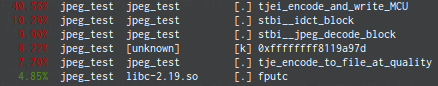
\includegraphics[width=4.5625in]{fputc}
    \caption{TinyJPEG: 48\%. fputc: 4.8\%}
\end{figure}

Este reporte de la herramienta \verb+perf+, parte de Linux Perf Tools
\cite{linux-perf-tools}, es de un programa de prueba que carga una imagen de
Plutón de 192 MB y la codifica con TinyJPEG. Lo que se muestra es que hay dos
funciones de TinyJPEG consumiendo el 48.2\% del tiempo. También muestra que la
función \verb+fputc+ consume 4.8\% del tiempo total. Con esto concluímos que si
solo tomamos en cuenta el tiempo que se pasa codificando la imagen, se está
gastando el 9.1\% del tiempo llamando a fwrite, (que a su vez llama a putc).

No se incluye un reporte de TinyJPEG con \emph{buffering} porque al usar un
buffer de 1024 bytes, eliminamos por completo el costo de \verb+fwrite+.

\subsection{CPU: Saltos condicionales}\label{sub:cpu-branch}

Para terminar las notas de micro-optimización, se va a discutir un truco en la
implementación de TinyJPEG que trata con predicción de \emph{branches} (i.e.
saltos condicionales, o bloques \verb+if+)

Los CPUs son muy buenos ejecutando \emph{branches} cuando pueden predecir su
comportamiento. Agner Fog \cite{agner} tiene muy buenos recursos para estar al
día con la manera en que los procesadores de Intel predicen branches. El
concepto es que cuando el CPU piensa que un branch va a ser ejecutado, lo
ejecuta \emph{ especulativamente } mientras la condición del salto se computa
paralelamente. Se le conoce como un \emph{branch missprediction}, que
traducimos como \emph{mis-predicción de salto} a la situación en cuando el
salto se calculó especulativamente pero la condición falló. En código de alto
desempeño como la función interna de JPEG, esto puede ser un cuello de botella.

En el caso e TinyJPEG, una vez que se utilizó un algoritmo rápido de DCT, el
cuello de botella en la función \verb+encode_MCU+ resultó ser la siguiente
línea de código:

\begin{code}[language=C][h]
fval = (fval > 0)? floorf(fval + 0.5f) : ceilf(fval - 0.5f);
\end{code}

Esta es una implementación clásica de redondeo, escrita de acuerdo a la
especificación JPEG.

Usando \verb+perf+, se puede visualizar el problema:

\begin{figure}[hb]
    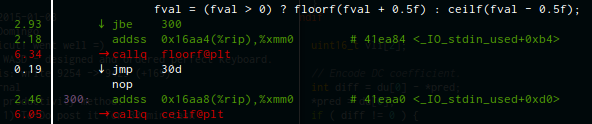
\includegraphics[width=5.16666in]{round_slow}
    \caption{Mis-predicción de salto}
\end{figure}

Ambos caminos del salto condicional inducido por el operador \verb+?:+ toman
alrededor de 9 ciclos de CPU, con un total de 18. En el momento en que se
encontró este problema, 18 ciclos de reloj en \verb+encode_MCU+ eran un cuello
de botella.

Esa información no es suficiente para decidir que el problema es
mis-predicción, pero se puede atacar al problema aplicando la medicina y
realizando un diagnóstico si resulta efectiva.

En este caso, sabemos que $fval \in [-1024, 1024]$. Esta información nos
permite evitar el salto haciendo una suma, $(fval + 1024) \in [0, 2048]$. Si
hacemos esto, podemos usar \verb+floorf+, ya que el valor siempre es positivo:

\begin{code}[language=C][h]
    fval += 1024;
    fval = floorf(fval + 0.5f);
    fval -= 1024;
\end{code}

El resultado, con \verb+perf+:

\begin{figure}[hb]
    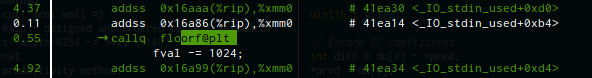
\includegraphics[width=5.16666in]{round_fast}
    \caption{Evitando mis-predicción}
\end{figure}

Como logramos alrededor de 2X de mejora en velocidad, podemos concluir con
confianza que el salto no se estaba prediciendo exitosamente, con el resultado
de que \verb+floorf+ y \verb+ceilf+ se estaban calculando \emph{siempre},
independientemente de si \verb+fval+ era positivo o negativo.



